%\thispagestyle{intro}

% \section*{Conventions}
% \phantomsection
% \addcontentsline{toc}{section}{\protect\numberline{}Conventions}
\invisibleunnumberedchapter{Conventions}%

\e
    \item Organisation du document:

    {\Large Chapitre} {\large Section} Sous-section {\small Sous-sous-section}

    \item Organisation des paragraphes:

    {\Large a} . {\large 1} . (a) . {\small (1)}
    
    \item Lien interne en \textcolor{black!60}{gris}:
    
    \fullref{preparation}
    
    \item Lien externe en \textcolor{blue!60}{bleu}:
    
    \thirdwing    

    \item Exemple tiré du \jp{}:

    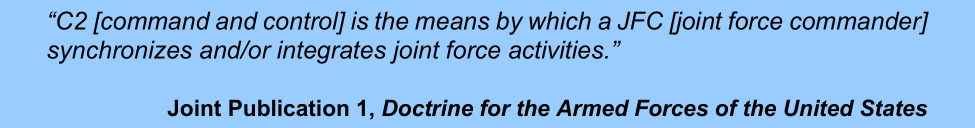
\includegraphics[width=0.7\paperwidth]{jptextex.png}

    \item Image tirée du \jp{}:

    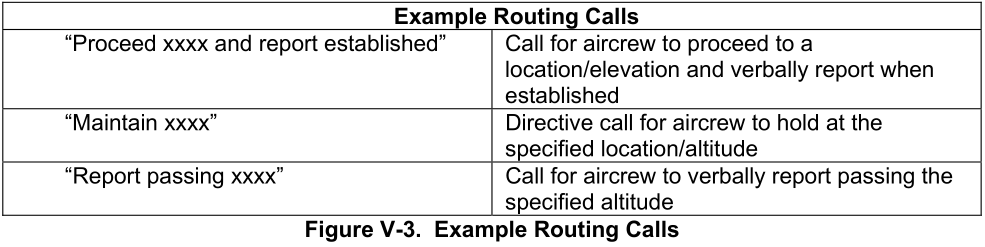
\includegraphics[width=0.7\paperwidth]{routing.png}

    \item Communication radio:
    \begin{lstlisting}
        Sochi sol, REDWOLF, pour la mise en route
        REWOLF, Sochi sol, QNH 0758, vent calme, mise en route approuv"é"e, rappelez pr"ê"t "à" rouler
    \end{lstlisting}

    \item \textbf{Emphase forte.}

    \item \emph{Emphase légère.}

    \item \important{Information importante.}
    
    %\item \useful{Information utile.}
    
    \item \remark{Remarque ou ensemble cohérent.}

    \item \note{Contenu, suggestion ou opinion qui n'est pas extrait du \jp{}.}

\ed 